\chapter{System Validation}\label{ch:validation}

\textcolor{red}{THIS IS AN UNFINISHED CHAPTER}

This chapter presents the validation of the proposed solution.
The validation process is described into different sections, each addressing different components of the system.
Section~\ref{sec:meth} outlines the methodology used for validation.
Section ~\ref{sec:experimental-setup} presents the experimental setup.
In Section ~\ref{sec:component-testing}, each component is tested.
\textcolor{red}{UPDATE ACCORDINLY}
Section~\ref{sec:use_case} presents a specific use case to demonstrate the system's functionality.
Finally, Section~\ref{sec:discuss} provides a discussion of the results and insights gained from the validation process.

\section{Methodology}\label{sec:meth}
We have divided our tests into three categories: Component Testing, Interoperability Testing and Use Case Validation.
The first was used to validate the proper functioning of each component, with a performance evaluation when possible.
The second category serve to determine if the components were working jointly properly.
The last seek to validate the proposed system in a reference scenario.
In each set of tests, we conducted a functional validation using tools such as ping and Iperf~\cite{iperf}.
When applicable, the performance was evaluated.
\textcolor{red}{Maybe write something more}

\section{Experimental Setup}\label{sec:experimental-setup}
This section presents the experimental setup.
Figure~\ref{fig:setup} shows a photograph of the experimental scenario.

\begin{figure}[H]
    \centering
    
\includegraphics[width=0.5\linewidth]{figures/uporto-feup}
    \caption{Experimental setup}
    \label{fig:setup}
\end{figure}


\section{Component testing}\label{sec:component-testing}


\subsection{Core Network}\label{subsec:core_network}
In this section, the Core Network configuration and validation are discussed.
It includes the setup of network elements, their interactions, and performance metrics.
In order to make sure that all Core Network components are working properly, we performed a test.
The deployment of the Core Network is done through Docker containers.
Figure~\ref{fig:core_init} presents the command for running the Core Network setup script.
After the initialization of the Docker containers, it is possible to see the logs of the setup script, indicating the successful initialization.

\begin{figure}[H]
    \centering
    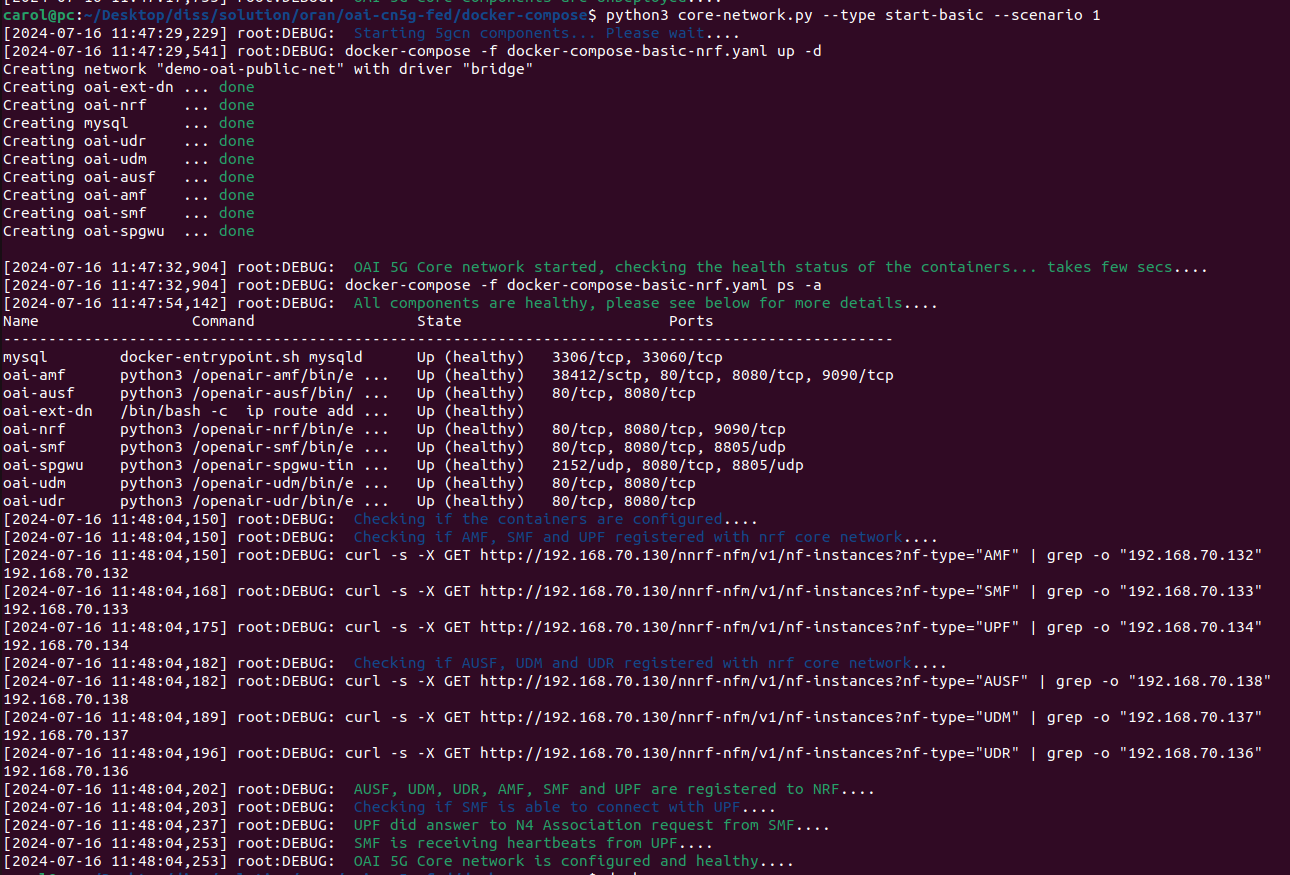
\includegraphics[width=0.5\linewidth]{figures/core_init}
    \caption[Initialization of the Core Network]{Initialization of the Core Network}
    \label{fig:core_init}
\end{figure}

In order to confirm the correct deployment, the interface \textit{demo-oai} must appear when running the \textit{ifconfig} command.

Then, we verified that all the containers had connectivity using the interface created in the Host OS, using the ping tool,as shown by Figure~\ref{fig:ping_core}.
Each interface sends requests to each network component according to the table~\ref{tab:ip_core}.

\begin{figure}[H]
\centering

\includegraphics[width=0.5\linewidth]{figures/uporto-feup}
\caption[Pinging NRF, MySQL Database, AMF, SMF, UPF, UDR, UDM and AUSF respectively from Host OS
interface]{Pinging NRF, MySQL Database, AMF, SMF, UPF, UDR, UDM and AUSF respectively from Host OS
interface}
\label{fig:ping_core}
\end{figure}


Successfully concluding this tests ensures that the 5G Core Network is operational.

\section{FleXRIC}\label{sec:flexric}
As for the FlexRIC deployment, it is simply necessary to assure its correct launch.
Upon launching, it awaits for incoming connection requests from an E2 Node.
Figure~\ref{fig:near-rt-ric} shows the initialization of the FlexRIC\@.

\begin{figure}[H]
    \centering
    
\includegraphics[width=0.5\linewidth]{figures/uporto-feup}
    \caption{Initialization of FlexRIC's executable}
    \label{fig:near-rt-ric}
\end{figure}

When it is properly launched, the gNB can be initialized.

\section{gNB}\label{sec:gnb}
\textcolor{red}{Finish}
To ensure the correct functioning of the gNB, it should be registered in the 5G Core Network, connected to the FlexRIC and registered as a E2 node.
They need to be validated separately since the connections are independent.

To access the gNB connectivity to the Core, we need to check the connection between the gNB Host and the AMF and UPF, since the gNB needs to communicate with them.
This can be tested with ping from the gNB's Host to these entities.
Figure~\ref{fig:ping_gnb} shows the results.

% figure with ping to AMF and UPF 132 and 134

\begin{figure}[H]
    \centering
    
\includegraphics[width=0.5\linewidth]{figures/uporto-feup}
    \caption{Conection test to AMF and UPF, respectively, from gNB Host.}
    \label{fig:ping_gnb}
\end{figure}

After

\section{UE}\label{sec:ue}
\textcolor{red}{Finish}

In order to test the correct initialization of the UE we needed to ensure connection with the Core Network.
After executing the command present in~\ref{subsec:oai-5g-ue}, we observed in Wireshark the correct registration of the UE in Figure~\ref{fig:registration_ue}.

\begin{figure}[H]
    \centering
    
\includegraphics[width=0.5\linewidth]{figures/uporto-feup}
    \caption{Registration of the UE}
    \label{fig:registration_ue}
\end{figure}

When this synchronization occurs, we can verify the creation of \textit{oaitun\_ue1}, the tunnel interface between UE and Core Network.
With that, we can test its connectivity, by pinging to every Core Network component, as well as the Internet.
Figures~\ref{fig:ping_ue_core} and~\ref{fig:ping_ue_internet} shows the outcome of these tests, to Core and to the Internet respectively.

\begin{figure}[H]
    \centering
    
\includegraphics[width=0.5\linewidth]{figures/uporto-feup}
    \caption{Pinging from UE to the Core Components}
    \label{fig:ping_ue_core}
\end{figure}

\begin{figure}[H]
    \centering
    
\includegraphics[width=0.5\linewidth]{figures/uporto-feup}
    \caption{Pinging from UE to Google's public DNS server}
    \label{fig:ping_ue_internet}
\end{figure}




\section{Computer Vision Module}\label{sec:cv_module}
To ensure the correctness and reliability of the computer vision module, a series of validation tests were conducted.
These tests were designed to evaluate both the processing capabilities of the module and the accuracy of the message exchange between the vision module and the xApp.

The processing time of each frame was measured to assess the real-time performance of the computer vision module.
This is important to ensure that the module could keep up with dynamic environments, such as an office setting where people and objects are constantly moving.
The tests showed that the processing times were within acceptable limits, allowing for timely detection and response.
% show some math on why this result is sufficient
% plot some results

A reference video was used to evaluate the detection and tracking results of the computer vision module.
This video, containing typical office movements like people walking and objects being moved, was processed to check for detection accuracy and tracking consistency.
The results confirmed that the module could accurately detect and track objects, validating its effectiveness in a real-world scenario.
Figure~\ref{fig:reference_video} shows the

% image of a frame of the video and the corresponding messages
\begin{figure}[H]
    \centering
    
\includegraphics[width=0.5\linewidth]{figures/uporto-feup}
    \caption{Reference video and corresponding messages generated.}
    \label{fig:reference_video}
\end{figure}

Print statements were used on the server side to verify the correct formatting, coding, and decoding of the messages.
This step was crucial to ensure that the messages sent from the computer vision module to the xApp were correctly structured and could be properly interpreted upon receipt.

On the client side,the xApp, print statements were employed to confirm the correct reception of the messages.
This validation step ensured that the messages transmitted through the socket connection were received intact and could be  correctly processed.

To further validate the communication, Wireshark was used to capture SCTP packets containing the messages exchanged between the server and client.
This capture provided a detailed view of the message flow, confirming that the messages were being transmitted as expected without any loss or corruption.
The capture presents the

% image of the wireshark capture

% MEASURE IF THE SCTP MESSAGES ARE BOTTLENEKING THE APPLICATION.

% maybe define a periodicity for it.


The computer vision module's performance proved adequate for the intended application, i.e.\ an office environment where movements are frequent yet the velocity is low, such as people walking or objects being moved.
The module demonstrated good performance in these scenarios, and its near real-time processing capability can ensure prompt reactions to environmental changes.



\section{xApp}\label{sec:mm_xapp}
This section focuses on the Mobility Management xApp and its role in the system.
It details the design and implementation of the xApp, how it interfaces with other components, and the results of its validation.

\section{Use case}\label{sec:use_case}
In order to validate the implemented solution, a use case testing scenario was established.
In an indoor environment, the system followed the architecture presented in Figure~\ref{fig:}.

The goal of test was to access the functionality of the whole system, considering maintaining end-to-end connection between the UE and the external DN. The Mobile RAN positioning is defined by the mobility management xApp, based on data collected from the Computer Vision Module and the radio metrics collected from the RAN via the Near-RT RIC. It aimed at maintaining the channel quality, or increasing it whenever possible.

The use case shows the system's capabilities in three test scenarios, described in the following subsections.

For all scenarios we are assuming constant velocity for all moving entities.

\subsection{Scenario 0 : Fixed gNB and UE}\label{subsec:scenario-0-:-fixed-gnb-and-ue}

In this scenario, the objective is to assess the impact of blockages on the LoS between the gNB and the UE\@.
By maintaining a fixed position for both the gNB and the UE, we can introduce obstacles to observe their effects on signal quality.
This scenario also aims to validate the accuracy of the messages sent by the vision module regarding the presence of blockages.
Figure~\ref{fig:test_fixed} presents a top-view from the testing scenario.
The obstacle moves from left to right, over time at a constant velocity.

The results from this scenario serve as a baseline for comparison with other scenarios, where the positions of the gNB and UE may vary.
This analysis is important for evaluating the gains of having computer vision solutions integrated into mobile networks.

\begin{figure}[H]
    \centering
    
\includegraphics[width=0.5\linewidth]{figures/uporto-feup}
    \caption{Overview of scenario}
    \label{fig:test_fixed}
\end{figure}

\begin{figure}[H]
    \centering
    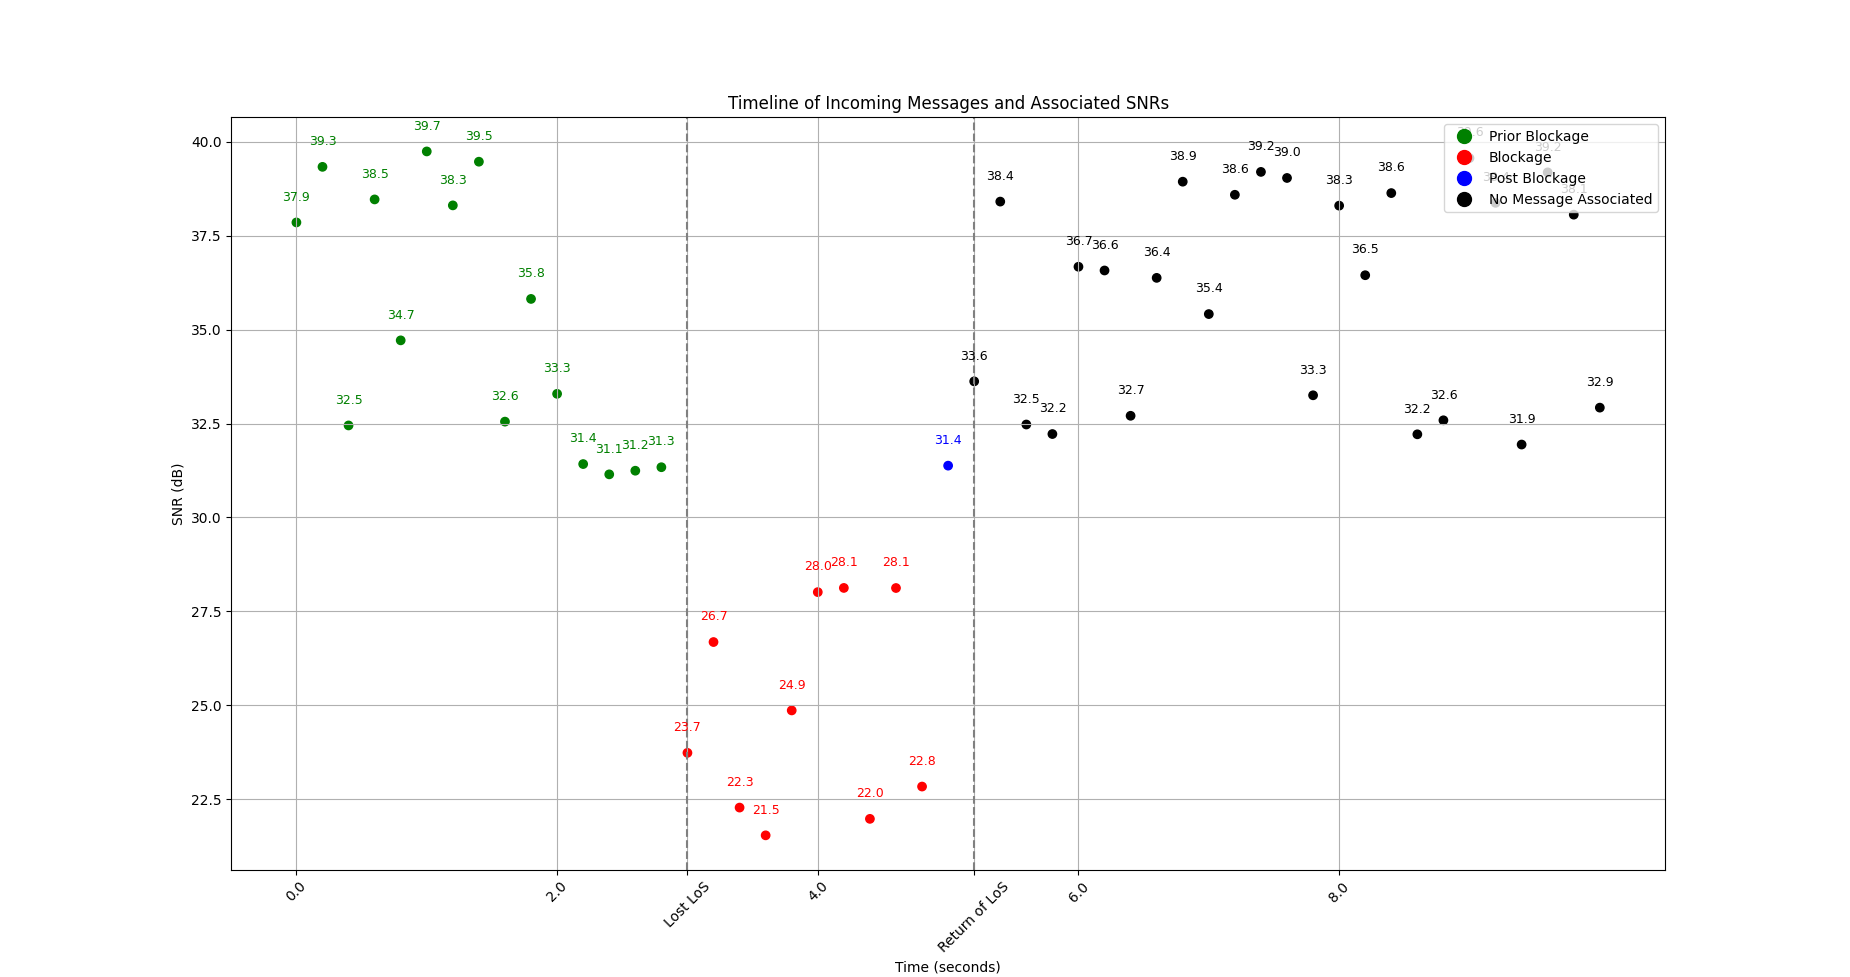
\includegraphics[width=\linewidth]{figures/dummy results}
    \caption{Dummy results}
    \label{fig:results_0}
\end{figure}


This test was successful, showcasing the CV module messages received, as well as SNR metrics corresponding to those expected.

Figure~\ref{fig:results_0} presents the graph with the results collected from this experiment.
It is possible to see the SNR variation over time in the y-axis , associated with each message, over a period of 10 seconds.
The average SNR values are collected by the xApp in intervals of 200 milliseconds (20 sample collected over a period of 10ms).
Possible values for this collection of data are 1ms,2ms, 5ms or 10ms.
This value is set according to the estimated fps of the video.
Since prior test has shown that capturing in 30fps results in the processing of video of about 5fps, we chose this value so that each message reception will have an SNR associated.
Each message is represented by a colour, as shown in the legend.
Notice that we can also have situations were we have SNR data collection but no associated message, for instance when no obstacles are detected or when the obstacles seen are not expected to block the LoS\@.

The graph is divided into three distinct stages, separated by the transition lines.
In the first stage, where the obstacle is moving towards the UE, Prior Blockage messages are sent.
The SNR is high (above 30dB) since there are no obstruction of LoS between gNB and UE, indicating a strong and clean signal.

The first transition at X seconds is labeled \("\)Lost LoS\("\).
This marks the beginning of the blockage period.

In the second stage,the obstacle stops in front of UE,
and it is possible to see the reception of the first Blockage Message, indicating the beginning of such obstruction.
As expected, the average SNR lowers.

The second transition at X seconds is labeled **\("\)Return of LoS\("\)**, indicating the end of the blockage and the return to normal signal conditions.
In the third stage, the obstacle moves away from the UE, no longer blocking the LoS\@.
As expected, the average SNR approximate those seen in the first stage.
The SNR values return to above 30 dB, similar to the prior blockage stage, indicating the restoration of a clear and strong signal, suggesting the removal or resolution of the blockage.

In this scenario, we also have used iperf tool to test the throughput in two instants.
The first one was when no blockage was occurring.
The second on was when a blockage was ongoing.
As expected, the throughput is lower when there is a blockage.
Table~\ref{tab:iperf} presents the measured values.


\begin{table}[h]
    \centering % Center the table
    \begin{tabular}{|c|c|c|c|}
        \hline
        \textbf{Instant} & \textbf{Connection type} & \textbf{DL} & \textbf{UL} \\ \hline
        \multirow{2}{*}{No blockage} & UDP & & \\ \cline{2-4}
        & TCP & & \\ \hline
        \multirow{2}{*}{Blockage}    & UDP & & \\ \cline{2-4}
        & TCP & & \\ \hline
    \end{tabular}
    \caption{Iperf results} % Add a caption for the table
    \label{tab:iperf} % Add a label for referencing the table
\end{table}






\subsection{Scenario 0.1: Fixed gNB, moving UE}\label{subsec:scenario-0.1:-fixed-gnb-moving-ue}
This scenario also aimed at evaluating the

This test occurred as expected.
We noticed that the CV module generated wrong messages specially when it came to Pior Blockage messages, as anticipated.
This is due to the fact that the module has no notion of depth.

\subsection{Scenario 0.1: Fixed gNB, moving UE, Obstacle present}\label{subsec:scenario-0.1:-fixed-gnb-moving-ue-obstacle-present}

This scenarios aims at evaluating the accuracy of the messages generated.
It also aims at showcasing the multi obstacle capacity of the bot-SORT model and how it interferes with the messages generated by the vision module..

\subsection{Scenario 1: Moving gNB}\label{subsec:scenario-1:-moving-gnb}
% change it
In this scenario, the User Equipment (UE) encounters an obstacle that obstructs its line of sight. % change specially this sentance
The system promptly identifies the obstacle and predicts when the blockage is expected to happen.
A message indicating the future blockage is sent to the xApp, which then informs the gNB (gNodeB). In response, the gNB preemptively adjusts its position to maintain a clear line of sight with the UE, thereby sustaining a consistent average Signal-to-Noise Ratio (SNR). This proactive approach ensures uninterrupted communication and optimal performance despite the presence of obstacles.

%\subsection{Scenario 2: UE Moving Away from the gNB}\label{subsec:scenario-2:-ue-moving-away-from-the-gnb}

%This scenario involves the UE moving progressively further from the gNB. In the absence of identified obstacles, a decrease in the Signal-to-Noise Ratio (SNR) is interpreted as the UE increasing its distance from the gNB. To address this, the robotic platform, leveraging the Mobility Management xApp, dynamically moves towards the UE to uphold optimal communication quality.
%This adaptive response ensures that the UE remains within the effective communication range of the gNB, thereby maintaining robust and reliable connectivity.


\section{Discussion}\label{sec:discuss}
This section provides a discussion on the results obtained from the validation process.
It includes insights, lessons learned, and potential areas for improvement in future iterations of the system.
